\documentclass{article}

\usepackage{amsmath}
\usepackage{braket}
\usepackage{amssymb}
\usepackage{tikz}
\usepackage[nottoc]{tocbibind}
\usepackage{graphicx}
\usepackage[backend=bibtex,style=numeric]{biblatex}
\bibliography{sample}
\begin{document}
\tableofcontents
\newpage
%\begin{tikzpicture}
    %\clip (-1,-1) rectangle (3cm,2cm); 
  %  \draw[very thick] (0,0) grid[step=1cm] (3,2);

    %\foreach \x in {0,1,2,3}
   %{
     %   \foreach \y in {0,1,2}
       % {
         %   \node[draw,circle,inner sep=3pt,fill] at (1*\x,1*\y) {};
        %}\\
    %}
%\end{tikzpicture}

\section{Introduction}
Lattice model thought to describe relevant microscopic details from
which macroscopic properties can be derived.

The linked cluster expansion (LCE) is a systematic approximation of quantum
lattice models in the thermodynamic limit. It is based on the fact
that an extensive quantity can be expressed by the sum over all
connected, or linked clusters that can be embedded in the lattice
\cite{Series,Rigol}. The value of each cluster can be calculated in
several ways, e.g. by perturbation theory \cite{Series} or numerically
by exact diagonalization, as in this thesis.

We apply the NLCE to the transverse field Ising model (TFIM) in order to
calculate ground state properties, like the magnetization.

This thesis is made up as follows. We first give a short introduction
to the transverse field Ising model, then we discuss exact
diagonalization for TFIM in one and two dimensions. Following that the
LCE is discussed and its implementation using $n \times m$ rectangles
is described. Finally we discuss the simulations and give an outlook
on how to progress from there.

\newpage


\section{Transverse Field Ising Model}
The Ising model is one of the simplest toy model of magnetism. It is
made up of spins $\sigma_i$ on a lattice, that can either point up or
down and can interact with neighboring spins and a external magnetic
field h.
\begin{equation}
\label{eq:18}
\mathcal{H} = -J \sum\limits_{\langle i,j \rangle} S_i S_j- h
\sum\limits_i S_i
\end{equation}
In this thesis we consider the Ising Model in an external magnetic
field, that is perpendicular to the interaction term $-J \sum_{\langle
i,j \rangle} \sigma_i \sigma_j$, from now on called the transverse
field ising model (TFIM). We therefore have to replace the $S_i$ with
the familiar Pauli matrices $\sigma^x$ and $\sigma^z$.
\begin{align}
\label{eq:14}
\mathcal{H} &= \mathcal{H}_0 + \mathcal{H}_1
\end{align}
\begin{align}
\label{eq:24}
\mathcal{H}_0 &= -J \sum\limits_{\langle i,j \rangle} \sigma_i^z \sigma_j ^z\\
\mathcal{H}_1 &= - h \sum\limits_i \sigma_i^x
\end{align}
Where the first sum runs over all pairs of nearest neighbors. If the
system has open boundary conditions, as is the case for this thesis and consists of N spins, then
\eqref{eq:14} simplifies to:
\begin{equation}
\label{eq:19}
\mathcal{H} = -J \sum\limits_i^{N-1} \sigma_i^z \sigma_{i+1} ^z- h
\sum\limits_i^N \sigma_i^x
\end{equation}
\\
Notice that the TFIM, unlike the Ising Model, has to be described
quantum mechanically, because $\mathcal{H}_0$ and $\mathcal{H}_1$ do
not commute .

\section{Exact Diagonalization}
We want to solve the Schr\"odinger Equation.
\begin{equation}
\label{eq:1}
\mathcal{H} \ket{\psi} = E \ket{\psi}
\end{equation}
But most of the time it is not possible to solve the Schr\"odinger
Equation analytically, therefore one has to resort to numerical
approaches.\\
For a finite dimensional system $\mathcal{H}$ is an hermitian matrix
and we want to find the eigenvalues and corresponding eigenvectors of $\mathcal{H}$.
This task of finding all or only some of the eigenvalues and
eigenvectors is commonly referred to as exact diagonalization.\\
Thermal expectation values can then be calculate using, e.g. the
canoncial ensemble, but other ensemble are, of course, also possible:
\begin{equation}
\label{eq:2}
\braket{A} = \frac{ \text{Tr}(Ae^{-\beta \mathcal H})}{ \text{Tr}(e^{-\beta \mathcal
    H})} = \frac{\sum\limits_i e^{-\beta
      E_{i}} \braket{\psi_i|A|\psi_{i}}}{\sum\limits_i e^{-\beta
      E_i} \braket{\psi_i|\psi_{i}}} = \frac{\sum\limits_i A_i e^{-\beta
      E_{i}}}{\sum\limits_i e^{-\beta
      E_i}}
\end{equation}
Here E$_{i}$, $\ket{\psi_i}$ are the eigenvalues and  eigenvectors of
the Hamiltonian $\mathcal{H}$, respectively and $A_i$ are the
eigenvalues of the operator $A$.If $A$ is diagonal in the same basis as
the hamiltonian, then one only has to diagonalize the hamiltonian and
perform the sum, but $A$ does not have to be diagonal, thus one must
diagonalize $A$ in the same basis as $\mathcal{H}$.\\
There, of course, exist other methods
of calculating partition functions, e.g. monte carlo based methods but they
are conceptually not as simple.

Exact diagonalization is an exact method of calculating properties,
because no further simplifying assumptions are made after the
hamiltonian has been derived.\\
The downside of exact diagonalization is that $\mathcal{H}$ grows
exponentially with the number of sites, e.g. for the TFIM
$\mathcal{H}$ is $2^N \times 2^N$ dimensional, where N is the number
of lattice sites. In practice one is limited to very
few particles, up to roughly 40 on a 2D lattice \cite{Noack}.\\
Such large system sizes can only be achieved by making use of the
symmetries of the Hamiltonian, whereby the Hamiltonian is blockdiagonal
(and thus smaller)
under the action of its symmetry group. This theorem is due to Wigner
and Eckart. The TFIM does not
have any symmetries that can be used to reduce the matrix dimension,
therefore we refer the reader to the literature
\cite{Laflorencie,Noack,Fehske}.\\
On the upside on can calculate, at least in principle, any quantity,
both static and dynamic, because one has access to the whole
wavefunction \cite{Noack}.\\
The basic idea is then to set up the hamiltonian in some basis and
then diagonalize it using a computer. If one is only interested in
extremal eigenvalues and eigenvectors, like the ground state, then one
does not have to diagonalize the whole matrix, but one can then find
them using an iterative diagonalization procedure like the Lanczos
algorithm \cite{Lanczos}, which is a lot faster and allows one to treat much larger
systems. In this thesis a lanczos based eigenvalue solver is used.\\

\subsection{Basis Construction}
\subsubsection{1D Model}
The hamiltonian is in operator form, in order to diagonalize it one
has to convert it to matrix form. In principle one can use any basis,
for the spin 1/2 systems like the Ising model it is most convenient to
work in the $\sigma^z$ basis \cite{Noack,Laflorencie}.\\
We use the identification $\ket{\uparrow} = \ket{1}$ and $\ket{\downarrow} = \ket{0}$. One can then write a many-body state in the following form: $\ket{\uparrow \uparrow \dotso \downarrow} = \ket{11 \dotso 0}$. In this thesis, the states are numbered from the right side and we count from zero upwards, that is the rightmost state is the zeroth spin.\\
In order to set up the matrix one has to generate a complete basis, e.g. one has to create all 2$^{N}$ combinations of $\uparrow$ and $\downarrow$ spins.\\
For $N=2$ sites this corresponds to:
\begin{align*}
&\ket{\downarrow \downarrow} = \ket{00}\\
&\ket{\downarrow \uparrow} = \ket{01}\\
&\ket{\uparrow \downarrow} = \ket{10}\\
&\ket{\uparrow \uparrow} = \ket{11}\\
\end{align*}
Furthermore it is necessary to determine the action of the Hamiltonian on the basis states.\\
The TFIM Hamiltonian consists of two different parts:
\begin{align}
\label{eq:5}
\mathcal{H}_0 &= -J \sum\limits_{i}\sigma_i^z\sigma_{i+1}^z\\
\mathcal{H}_1 &= -h \sum\limits_i^{}\sigma_i^{x}
\end{align}
Where the $\sigma_i$ are Pauli matrices , whose action on the basis states is defined as follows:
\begin{align*}
\sigma^z \ket{\uparrow} &= 
\begin{pmatrix}
1 & 0\\
0 & -1
\end{pmatrix}
\begin{pmatrix}
1\\
0
\end{pmatrix} = 
\begin{pmatrix}
1\\
0
\end{pmatrix} = \ket{\uparrow}
\\
\sigma^z \ket{\downarrow} &= 
\begin{pmatrix}
1 & 0\\
0 & -1
\end{pmatrix}
\begin{pmatrix}
0\\
1
\end{pmatrix} = -
\begin{pmatrix}
0\\
1
\end{pmatrix} = -\ket{\downarrow}
\\
\sigma^x \ket{\uparrow} &= 
\begin{pmatrix}
0 & 1\\
1 & 0
\end{pmatrix}
\begin{pmatrix}
1\\
0
\end{pmatrix} = 
\begin{pmatrix}
0\\
1
\end{pmatrix} = \ket{\downarrow}
\\
\sigma^x \ket{\downarrow} &= 
\begin{pmatrix}
0 & 1\\
1 & 0
\end{pmatrix}
\begin{pmatrix}
0\\
1
\end{pmatrix} =
\begin{pmatrix}
1\\
0
\end{pmatrix} = \ket{\uparrow}
\end{align*}
That generalizes straightforwardly to the many-body basis: $\sigma_i^z
\ket{\dotso \uparrow_{i+1} \downarrow_i \dotso} = - \ket{\dotso \uparrow_{i+1} \downarrow_i\dotso} $ Then $\mathcal{H}$ is applied to every basis state, in order to set up the matrix.\\The resulting matrix is sparse, that is it contains mostly zeros and we can save a lot of memory by only saving the nonzero elements.\\
As one can see, applying $\mathcal{H}_0$ to a basis state always yields the same state, thus $\mathcal{H}_0$ is diagonal in this basis.\\
For the 3 site chain, $\mathcal{H}_0$ acts the following way on a state:
\begin{align*}
\mathcal{H}_0 \ket{\uparrow \downarrow \uparrow} = -J(\sigma_0\sigma_1 + \sigma_1\sigma_2) \ket{\uparrow \downarrow \uparrow} = -J(-\ket{\uparrow \downarrow \uparrow} - \ket{\uparrow \downarrow \uparrow}) = 2J \ket{\uparrow \downarrow \uparrow}
\end{align*}
As one can see, one gets a + sign if two neighboring spins point in the same direction and a minus sign if they do not. Then one has to simply count the number of plus and the number of minus signs and subtract them.
If the application of $\mathcal{H}_0$ returns a nonzero state, we store it in a list, together with its multiple.\\
The application of $\mathcal{H}_1$  is not quite as simple. $\sigma_i^x$ flips the i'th spin, this can be accomplished with the exclusive or.
\begin{align*}
\sigma_0^x \ket{101} = \ket{001} XOR \ket{101} = \ket{100}
\end{align*}
To give an example:
\begin{align*}
\mathcal{H}_1 \ket{001} &= -h(\sigma_0 + \sigma_1 + \sigma_2)\ket{001} \\
&= -h(\ket{001}XOR \ket{001} + \ket{010}XOR \ket{001} + \ket{100}XOR \ket{001})\\
&= -h(\ket{000} +\ket{011} +\ket{101}) = -h(\ket{0} + \ket{3} +\ket{5})
\end{align*}
In the last step we have converted the binary number into its integer
representation, in order to find out which state was returned, this is
a simplified version of the more general method of condensing the
information of a string in a single number, called hashing and then searching for the
position of that number in the list of all basis states \cite{Zhang}.\\
Besides the integer representation, one can also use hash tables, binary search or look up tables. Which of those methods is best depends on the model and its symmetries.\\
Like before, we only save the position of the nonzero elements.Unlike $\mathcal{H}_0$, $\mathcal{H}_1$ is not diagonal, therefore we need to save both the column index, as well as the row index.\\
We take the column index to be the state H was applied to and as row
index the resulting states. In addition to that one has to store the value of h.\\
Finally one has to to combine both matrices, which can then be
diagonalized.\\
For the $N = 3$ case the matrix takes the following form:
\begin{equation*}
\label{eq:23}
H = 
\begin{pmatrix}
-2J & -h & -h &  0& -h & 0 &0 &0 \\
-h &0 &0 & -h &  0& -h & 0& 0\\
-h & 0& 2J & -h & 0& 0& -h &0 \\
 0& -h & -h&0 & 0& 0& 0& -h\\
-h &0 &0 &0 &0 & -h & -h &0 \\
 0& -h &0 &0 & -h & 2J &0 & -h\\
 0& 0& -h & 0& -h &0 &0 & -h\\
 0& 0& 0& -h & 0& -h & -h & -2J\\
\end{pmatrix}
\end{equation*}

\subsubsection{2D Model}
The 2D case is not quite as simple as the 1D case, because one has to
consider the geometry of the model.\\
The transverse field part of the hamiltonian gets done the same way as
\begin{equation}
\label{eq:25}
\mathcal{H}_1 = \sum\limits_i \sigma_i^x
\end{equation}
in the 1D case, because it acts on every spin, irrespective of
their neighbors.\\
On the other hand, one needs to consider the shape of the lattice for
the diagonal part, because it acts on neighboring sites. Thus the sum
needs to run over all bonds.
\begin{equation}
\label{eq:26}
\mathcal{H}_0 = \sum\limits_{\langle i,j \rangle} \sigma_i^z \sigma_j^z
\end{equation}
One can still use the same many body basis, but one needs to label the
states according to some convention \cite{Sandvik}. We consider a rectangular lattice
with $N = L_x \times L_y$ sites. Then a site can be labeled as $i =
x_i + y_iL_x$, where $(x,y)$ are the coordinates of the site, as
depicted in Figure \eqref{fig:1}.

\begin{figure}[htbp]
\centering
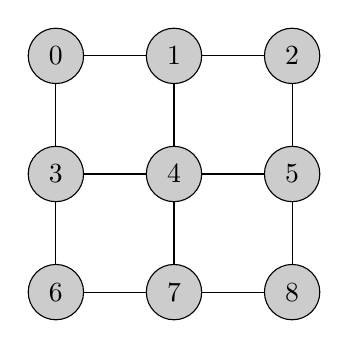
\begin{tikzpicture}[darkstyle/.style={circle,draw,fill=gray!40,minimum size=20}]
  \foreach \x in {0,1,2}
    \foreach \y in {0,1,2} 
       {\pgfmathtruncatemacro{\label}{\x - 3 *  \y +6}
       \node [darkstyle]  (\x\y) at (1.5*\x,1.5*\y) {\label};} 

  \foreach \x in {0,1,2}
    \foreach \y [count=\yi] in {0,1}  
      \draw (\x\y)--(\x\yi) (\y\x)--(\yi\x) ;

\end{tikzpicture}
\caption[]{\label{fig:1} site indices for the $3 \times 3$ square lattice}
\end{figure}
As for the $1D$ case, $\mathcal{H}$ is applied on every state and the
state, as well as $h$ and the resulting state get stored.



\subsection{Lanczos}
In order to find the eigenvalues of a N-dimensional Hamiltonian, one
has to find the roots to the characteristic polynomial of degree
$N$. Closed form solutions only exist for $ N\leq 4$ and for higher degrees
finding the roots is quite tricky.\\
Instead, one should find a unitary transformation that diagonalizes
the Hamiltonian:
\begin{align*}
H \to U^{\dagger} H U
\end{align*}
This can be done in an iterative way,
\begin{align*}
H \to U_1^{\dagger} H U_1 \to U_2^{\dagger}U_1^{\dagger} H U_1U_2 \to \dotsm
\end{align*}
This method is limited by the fact, that the whole Hamiltonian matrix
has to be stored and therefore the largest possible lattice size is
quite small.\\
If the ground state eigenvalue and eigenvector and low-lying excited
states are sufficent, then powerful iterative diagonalization
procedures, like the Lanczos algorithm, exist.

Those algorithms are all examples of the conceptually quite simple
power method \cite{Noack},
whereby one repeatedly applies the Hamiltonian to a random initial
state $\ket{v_0}$, which then converges towards the eigenvector of the
corresponding greatest (absolute) eigenvalue.
\begin{align*}
\ket{v_{n+1}} &= \frac{H \ket{v_n}}{\| H \ket{v_n} \|} =\frac{H^{n+1} \ket{v_0}}{\| H^{n+1} \ket{v_0} \|}  \qquad r_0 \in \mathbb{C}\\
\theta_n &= \frac{\braket{v_n|H|v_n}}{\braket{v_n|v_n}}
\end{align*}
Where $\theta_n$ converges towards the largest eigenvalue $\lambda$. The
subspace generated in the power method
 span\{$\ket{v},H \ket{v}, H^2 \ket{v}, \dotsc,H^n \ket{v}$\} 
is called the n'th Krylov space and forms the basis for many other
algorithms like the Lanczos method.

The Lanczos algorithm does not diagonalize the matrix, but brings it
in  triadiagonal form, which can then be diagonalized much easier \cite{Fehske}.
\begin{enumerate}
\item\label{item:1} Like before we start with a random vector
  $\ket{\phi_0}$, that is normalized\\
 $\|\phi_0\| = 1$
\item\label{item:2} apply H to this state
\item\label{item:3} orthogonalize these states with all previously
  generated states, in order to
  obtain a basis of the Krylov space, the matrix is tridiagonal in this basis
\item\label{item:4} go to 2 using the newly generated state, or end the
  recursion when the stoping criterion $\braket{\phi_{n+1}|\phi_{n+1}}
  < \epsilon$ is fulfilled 

\end{enumerate}
We can combined these steps in the following recursion relation \cite{Fehske}:

\begin{align*}
\ket{\phi'}&=H\ket{\phi_n} - \beta_n\ket{\phi_{n-1}}, \quad \text{with} \quad \ket{\phi_{-1}} = 0\\
\alpha_n &= \braket{\phi_n|\phi'}\\
\ket{\phi''} &= \ket{\phi'} - \alpha_n\ket{\phi_n}\\
\beta_{n+1} &= \|\phi''\| = \sqrt{\braket{\phi''|\phi''}}\\
\ket{\phi_{n+1}} &= \ket{\phi''}/\beta_{n+1}
\end{align*}\\
The resulting matrix T$_n$ has the form:\\
\begin{equation*}
T_n = 
\begin{pmatrix}
\alpha_0 & \beta_1 & 0 & &\\
\beta_1 & \alpha_1 & \beta_2 & 0 &\\
0 & \beta_2 & \alpha_2 & \ddots & \\
 & 0 & \ddots & \ddots & \beta_{n-1}\\
 & & & \beta_{n-1} & \alpha_{n-1}\\
\end{pmatrix}
\end{equation*}\\
The eigenvalues of T$_n$ converge to the eigenvalues of H if n is
large enough and typically 100 recursions are enough to come close to
machine precision for the ground state. Therefore one has to
diagonalize T$_n$, using for example the QR algorithm \cite{Francis1,Francis2}, which is a much
easier task than directly diagonalizing H.\\
Now that one has the eigenvalues and eigenvectors $\ket{\chi}$, with
components $\chi_j$, of
T$_n$ one can calculate the eigenvectors $\ket{\psi}$ of the original
hamiltonian H in the following way:
\begin{equation}
\label{eq:15}
\ket{\psi} = \sum\limits_{j=0}^{N-1} \chi_j \ket{\phi_j}
\end{equation}
This sum can be computed by repeating the lanczos procedure with
$\ket{\psi_0}$ as the start vector, omitting the scalar products for $\alpha_j$ and
$\beta_j$, which we already know \cite{Fehske}.\\
After the ground state has converged the vectors tend to lose
orthogonality due to finite machine precision.This is an intrinsic
limitation of the Lanczos method, which can be remedied by
reorthogonalizing all basis vectors as for example in the block-Lanczos
method, but one has to store all vectors in memory instead of just two
as described above. Furthermore there exist heuristic schemes like
Cullum-Willoughby \cite{Cullum2,Cullum}, but if one is only interested in a handfull of low
lying states, then the Lanczos method is often the preferred method of
choice \cite{Noack}.\\
An additional drawback is that it is impossible to resolve
degeneracies, for this one must use e.g. the band-Lanczos or the
Jacobi-Davidson algorithm \cite{Fehske}.\\ 

\section{Numerically Linked Cluster Expansion}
The linked Cluster Expansion is a method of calculating extensive properties of
a system in the thermodynamic limit, by extrapolating
from a series of finite size clusters, that can be embedded in the
lattice \cite{Rigol,Series,Domb}.\\
\subsection{High Temperature Expansion}

Calculating thermal properties of lattice systems is in general a
very difficult task. One possible way to do this, is to write the
partition function as a power series of the form $f(x) =
\sum_{n=0}^{\infty} a_nx^n$ and then calculate the coefficients $a_n$
for $n$ as large as possible. Expanding the partition function in terms
of the inverse temperature $\beta =
1/k_BT$ we get the high-temperatur expansion (HTE).
We demonstrate this for the Ising model:
\begin{equation}
\label{eq:10}
\mathcal{H} = -J \sum\limits_{\langle i,j \rangle} \sigma_i \sigma_j
\end{equation}
where the sum runs over all nearest neighbors. Then the canonical
partition function can be written as:
\begin{align}
\label{eq:11}
\mathcal{Z} &= \sum\limits_{\{ \sigma \}} e^{-\beta \mathcal{H}} =
\sum\limits_{\{ \sigma \}} e^{-K \sum_{\langle i,j \rangle}
  \sigma_i \sigma_j}, \quad with \quad K = \beta J\\
&= \sum\limits_{\{ \sigma \}} \prod\limits_{\left\langle i,j
  \right\rangle} e^{-K \sigma_i \sigma_j} =  \sum\limits_{\{ \sigma \}} \prod\limits_{\left\langle i,j
  \right\rangle} \sum\limits_{l = 0}^{\infty} \frac{K^l}{l!}(\sigma_i
  \sigma_j )^l
\end{align}
We can now express $(\sigma_i \sigma_j)^l$ graphically as an $l$-fold
bond between neighboring sites \eqref{fig:2}, thus one can write the partition
function in terms of graphs up to some maximum size
\cite{Rigol,Series}.\\
Equation \eqref{eq:11} implies, that it will only converge for high
temperatures, in other words $\beta$ must be greater or equal to $J$ \cite{Rigol}.

\begin{figure}[htbp]
\centerline{\includegraphics[scale = 0.5]{series_multigraph.png}}
\caption[]{\label{fig:2}  taken from \cite{Series}: we write the expansion in terms of the left
  hand side (LHS), by collapsing multiple bonds into single bonds}
\end{figure}

\subsection{Low-Temperature Expansion}
For systems close to their groundstate, i.e., for $\beta \to \infty$
we can write the partition function as:
\begin{equation}
\label{eq:12}
\mathcal{Z} = e^{-\beta E_0} \left( 1 + \sum\limits_{n \neq 0}
  e^{-\beta (E_n - E_0)} \right)
\end{equation}
where E$_0$ ist the groundstate. If there exists some energy
$\epsilon$, such that $m_n \epsilon = E_n - E_0$ , with $m_n \in
\mathbb{N}$, then one can write any thermodynamic property as a power
series in $e^{-\beta \epsilon}$. This can then be represented
graphically in terms of  graphs/clusters, just like for the HTE
\cite{Rigol,Series} and as with the HTE, the LTE does not converge at
any temperature but only for low temperatures.

\subsection{Linked Cluster Expansion}
The idea behind the linked cluster expansion (LCE) is to
express any extensive property, in the thermodynamic limit, as a sum
over all clusters $c$ that can be embedded in the lattice
\cite{Rigol}.\\
\begin{figure}[htbp]
\centerline{\includegraphics[scale=0.5]{site_based_rigol.png}}
\caption[]{\label{fig:3} taken from \cite{Rigol}: Some clusters that can be embedded on the
  square lattice. Clusters 3 and 5 are related by point-group symmetry and are topologically the same as cluster 4.}
\end{figure}\\
The extensive property $P(c)$ can be expressed by all contributions of
clusters that can be embedded in the cluster $c$.\\
\begin{equation}
\label{eq:9}
P(c) = W_P(c) + \sum\limits_{s \subset c} W_P(s)
\end{equation}
Where $W_P(c)$ is called the weight of a cluster $c$.
This can be rewritten as:
\begin{equation}
\label{eq:4}
W_P(c) = P(c) - \sum\limits_{s \subset c} W_P(s)
\end{equation}
The sum runs over all subclusters $s$ of $c$, that is each subcluster $s$ is
included the number of times it fits inside the cluster $c$ (Figure \ref{fig:sub}).
\begin{figure}[htbp]
\centerline{\includegraphics[scale = 0.5]{subclusters_melko.png}}
\caption[]{\label{fig:sub} taken from \cite{Melko}: The rectangular subclusters of a $2 \times 3$ cluster}
\end{figure}

One can then calculate $P/N$ in the thermodynamic limit by summing up
all weights \cite{Rigol}.
\begin{equation}
\label{eq:3}
P(\mathcal{L})/N = \sum\limits_c L(c) \times W_P(c)
\end{equation}
Here $L(c)$ is the number of possible embeddings per site for a cluster
$c$.\\
Due to the recursive definition of $W_P(c)$ contributions from
subclusters get canceled out, thereby accounting for boundary and finite-size effects.\\
A particularly nice fact about the LCE is that the sum converges for
different cluster geometries, as long as the subclusters can be
described in the same way. Thus one can choose the
building blocks that best fit the model one tries to solve. Possible building blocks for the square
lattice include the site,bond, square or n
$\times$ m rectangles based expansion and site, bond, or triangle
based expansion for the triangular lattice \cite{Rigol,Kallin}.\\
The general procedure for the LCE is to generate all clusters up to
some size, calculate their weights according to \eqref{eq:4} and then combine those
measurements in line with \eqref{eq:3}.\\
$P(c)$ can be calculated by any suitable method like perturbation theory
or numerically by exact diagonalization, as in this paper, or by the
density matrix renormalization group (DMRG), therefore justifying the name Numerically Linked Cluster
Expansion (NLCE). Furthermore we work with the canonical ensemble, but
other ensembles can also be used.\\
\begin{equation}
\label{eq:6}
P(c) = \frac{ \text{Tr} \left(\hat P(c) e^{-\beta \hat H_c} \right)}{ \text{Tr}
  \left(e^{-\beta \hat H_c} \right)}
\end{equation}
The NLCE enables one to work at any temperature, unlike the HTE and
the LTE, as long as the complete spectrum of a cluster is found.
\subsection{Connected Clusters}
The name linked cluster expansion comes from the fact that only
connected or linked cluster have to be considered, because the weight of two disconnected clusters is zero. This can be considered as a generalization of the
inclusion-exclusion principle, that states that $|A \cup B|$ is $|A|
+ |B| - |A \cap B|$, just as the number of elements in
the intersection of two disconnected sets is zero \cite{Melko}.\\
More explicitly, any extensive quantity $P(c)$, for two disconnected
clusters $c_1$ and $c_2$, can be written by the sum of its parts:
\begin{align}
\label{eq:7}
P(c) = P(c_1) + P(c_2), \qquad \text{where} \quad c = c_1 \cap c_2
\end{align}
But $c_1$, $c_2$ and their respective subclusters are both
subclusters of $c$, thus the weight of two disconnected clusters is zero
\cite{Rigol}.
\begin{align}
\label{eq:8}
W_P(c) &= P(c) - \sum\limits_{s \subset c} W_P(s)\\
&= P(c) - \left[ W_P(c_1) + \sum\limits_{s \subset c_1} W_P(s)
  \right]\\
&= P(c) - \left[ W_P(c_2) + \sum\limits_{s \subset c_2} W_P(s)
  \right]\\
&= P(c) - P(c_1) -P(c_2) = 0
\end{align}

\subsection{NLCE based on Rectangles}
The generation of all clusters and subclusters up to some size is, in
general, a computationally expensive task, that can be the
computational bottleneck when trying to calculate, e.g. groundstate
properties.\\
The generation of all clusters can be simplified by considering their
symmetry groups and topology. If the Hamiltonian preserves the underlying symmetry of the lattice,
then clusters related by point-group symmetries have the same weight
and can be grouped together. Furthermore even if two clusters are not
related by a point-group symmetry they still might be described by the
same Hamiltonian if the share the same topology (Figure \ref{fig:3}). Thus
one only has to diagonalize clusters that do not share the same
symmetry, are the same topologically, thereby reducing the amount of
clusters that must be diagonalized quite drastically \cite{Rigol}.
But even with the use of symmetries and topology, there are still
often too many clusters to enumerate, thus one can not use the full
potential of the cluster solver.\\
This issue can be sidestep by using an expansion based on $n \times m$
rectangles instead of the more familiar site or bond based
expansion for embedding on the square lattice. This is possible, since every bond- or site-based cluster
can be assigned to a unique rectangle. This significantly reduces the
number of sites needed to self-consistently define the sum and
generating all rectangles up to some order $l$ becomes a
trivial task that can be accomplished by a simple nested
loop \cite{Kallin}. Furthermore $L(c)$ can either be $1$ if $n=m$ or $2$ if $n
\neq m$.

To get a better grasp of the method, the $2 \times 2$ square lattice
is done explicitly. Here we consider $ n \times m$ rectangles separate from
$m \times n$ rectangles, thus $L(c) = 1$ for every rectangle.
\begin{align*}
W(1,1) &= P(1,1)\\
W(1,2) &= P(1,2) - 2W(1,1) = P(1,2) -2 P(1,1)\\
W(2,1) &= P(2,1) - 2W(1,1) = P(2,1) -2 P(1,1)\\
W(2,2) &= P(2,2) -2 W(2,1) -2 W(1,2) -4 W(1,1)\\
&= P(2,2) - 2 (P(2,1) -2
         P(1,1)) - 2(P(1,2) -2 P(1,1)) - 4 P(1,1)\\
&= P(2,2) -2 P(2,1) - 2 P(1,2) + 4 P(1,1)
\end{align*}
Then by summing up all clusters:
\begin{align*}
\label{eq:17}
P(\mathcal{L}/(2 \times 2) &=\sum\limits_c L(c) W_P(c) = \sum\limits_c
                      W_P(c)\\
 &= P(2,2) - P(2,1) - P(1,2) + P(1,1)
\end{align*}
\\
For the 1d chain, $P(\mathcal{L})/N$ simplifies to:
\begin{equation}
\label{eq:20}
P(\mathcal{L})/N = P(N) - P(N-1), \qquad N>1
\end{equation}
Explicit calculations for the $N \times M$ rectangles, with $N,M \geq 2$, hint at the fact that
\eqref{eq:3} might take the form:
\begin{equation}
\label{eq:21}
P(\mathcal{L})/(N \times M) = P(N,M) - P(N-1,M) - P(N,M-1) +
P(N-1,M-1)
\end{equation}
This has been shown to work for $N,M \leq 6$, but a general proof for
arbitrary $N$ and $M$ is still missing.

The rectangle based NLCE is particularly suited for the calculation of the
Renyi entanglement entropy \eqref{eq:16} for any $\alpha$, unlike
quantum monte carlo (QMC) and series expansion. Additionally it allows one
to separate the corner contributions from the contributions due to a
straight cut, which is also not possible with QMC \cite{Kallin,Melko}.\\
\begin{equation}
\label{eq:16}
S_{\alpha}(A) = \frac{1}{1-\alpha} \text{logTr}(\rho^{\alpha}_A)
\end{equation}
For $\alpha = 1$ we recover the more familiar von Neumann entanglement
entropy:
\begin{equation}
\label{eq:27}
S(A) = -\text{Tr}(\rho_A \text{log} \rho_A)
\end{equation}

\subsubsection{Finite Size Scaling}
Most of the time one studies systems with periodic boundary conditions, in
order to make use of translational symmetry, but even for large lattices,
finite size effects can still be there. It is possible to sidestep
this issue, by directly approximating the
thermodynamic limit, as with the NLCE.

Phase transitions are most often described in the thermodynamic limit by a non-analyticity in the
first or second order derivative of the free energy. But when one
simulates a system using a computer it is only possible to treat a
finite system, which is always analytic, because it only has finite degrees of
freedom. 

The task is then to extract the critical point and related quantities
from a finite system. Due to universality, the behaviour at a critical
point is often described by a power law, like $\mu = |t|^{-\beta}$. For the
finite system, of size $L$ this is thought to take the form
$\mu^{\star} = L^{-\beta
\nu} g(tL^{1/\nu})$, where $g$ is a scaling function (citations). Then
by varying parameters and fitting the results to $\mu^{\star}$ on e
can extract the critical values. This procedure is called finite size
scaling.

For the LCE one is directly approximating the thermodynamic limit,
thus one cannot use finite size scaling. But one can instead extract, e.g.
the critical point directly from the series. This can be done by the
method of Pade approximants, but other procedures are also possible.
The Pade approximants are defined as a ratio of two polynomials and
are used to asymptotically analyse a finite series.
\begin{equation}
\label{eq:34}
f(x) = \sum\limits_i^L a_i x^i = \frac{p_N(x)}{q_M(x)}
\end{equation}
Where $p_N$, $q_M$ are polynomials of degree $N$ and $M$, with $N + M
\leq L$.\\
By taking the derivative of the logarithm of f(x), one converts an
algebraic singularity into a simple pole. If f(x) takes the form $f(x)
= A(x)(x_c -x)^{-\theta}$, then
\begin{equation}
\label{eq:31}
D\text{log}f(x) = \frac{f'(x)}{f(x)} = \frac{A'(x)}{A(x)} +
\frac{\theta}{x_c - x} = \frac{p_N(x)}{q_M(x)}
\end{equation}
and one can then estimate the postion of $x_c$ from the roots of
$q_M(x)$ and the critical exponent $\theta$ from the corresponding
residues \cite{Series}.

The reader is encouraged to check out the literature on finite size
scaling and series analysis, as we will not use those methods in this thesis.

\section{Analysis}
\subsection{1D TFIM}
\subsubsection{Ground State Energy}
The energy at a temperature $T$ can be calculated as
\begin{equation}
\label{eq:28}
E = \braket{\mathcal{H}} = \frac{\sum\limits_i \epsilon_i
  e^{-\beta \epsilon_i}}{\sum\limits_i e^{- \beta \epsilon_i}}
\end{equation}
Where $\epsilon_i$ is the $i'th$ eigenvalue of $\mathcal{H}$. For the
ground state this simply reduces to
\begin{equation}
\label{eq:29}
E_0 = \epsilon_0
\end{equation}
Using the NLCE, this can be formulated as:
\begin{equation}
\label{eq:30}
P(\mathcal{L})/N = P(n) - P(n-1) = \epsilon_0^n - \epsilon_0^{n-1}
\end{equation}
where $\epsilon_0^n$ is the ground state of the $n$-site chain.

The 1D TFIM can be solved exactly \cite{Pfeuty}. The ground state
energy takes the form:
\begin{equation}
\label{eq:22}
E_0/NJ = - \frac{2}{\pi} (1+ \lambda)E(m)
\end{equation}
Where $\lambda = h/J$, $m= 4\lambda /(1+\lambda)^2$ and $E(m)$ is the
complete elliptic integral of the second kind. E(m) is singular at $m
= \lambda = 1$, which corresponds to a quantum critical point
\cite{Series}.

One can see that the grounds state energy per lattice site gets closer
to the exact solution as the number of sites gets increased, for both
ED and NLCE, as expected.



At low $h$, the NLCE is a lot closer to the exact result than ED, while for larger $h$
this advantage decreases, because the difference between
$\epsilon_0^n$ and $\epsilon_0^{n-1}$ shrinks as $h$ gets larger.
\begin{figure}[htbp]
\centerline{\includegraphics[scale=0.5]{energy.eps}}
\caption[]{\label{fig:energy-ed-nlce} }
\end{figure}



\subsubsection{Ground State Magnetization}
The expectation value of the magnetization $m_z = \sum_i^N \sigma_i^z$
is defined as:
\begin{align}
\label{eq:32}
\braket{m_z} = \braket{n|m_z|n} &= \sum\limits_{i,j} \chi_i \chi_j 
                                  \braket{j|m_z|i}\\
&= \sum\limits_i \chi_i^2 \braket{i|m_z|i}
\end{align}

Where $\ket{n}$ is an eigenvector of $\mathcal{H}$, with components $\chi_i$
\begin{equation*}
\label{eq:33}
\ket{n} = \sum\limits_i^N \chi_i \ket{i}
\end{equation*}
$m_z$ is diagonal in the $\sigma_z$ basis, that was used to set up the
hamiltonian, thus $\braket{i|m_z|i}$ counts the number of up spins and the number of
 downspins and returns their difference. For $h = 0$ when all spins
 point in the same direction $m_z$ is equal to the number of sites.

The magnetization can also be derived analytically \cite{Pfeuty} 
\begin{equation}
\label{eq:13}
m_z = 
\begin{cases} (1-\lambda^2)^{1/8} & \quad \lambda <1\\
0 & \quad \lambda >1
\end{cases}
\end{equation}

As for the ED case, when normalized to the number of sites, $m_z = 1$
for $h = 0$. This is due to the fact that $\sigma_i\sigma_j$ gives a
positive contribution when two neighboring spins align. The presence
of the external field then destroys this order and the magnetization
decreases until $h/J = 1$, where the phase transition happens.

For a finite system $\braket{m_z} = 0$, thus one must use a different
order parameter like the  absolute
magnetization $\braket{|m_z|}$, which is also valid in the
thermodynamic limit and that can be compared to the exact solution.

\begin{figure}[htbp]
\centerline{\includegraphics[scale=0.5]{mag.eps}}
\caption[]{\label{fig:mag} results come in pairs, like 10 and 11, rest
not shown}
\end{figure}

Near $h = 0$, both the NLCE and ED give accurate results, because
nearly all spins still point in the same direction. One can see then as $h$ is
increased, that the NLCE is a much better approximation of the
thermodynamic limit. For $h>1$ one gets much closer to the ideal value
$m_z = 0$ than with ED. Furthermore the sudden drop as one gets closer
to the singularity is also reproduced more faithfully.\\
The even terms of the NLCE give a much better result, then the uneven
terms. This comes from the fact, that the ED results come in pairs,
e.g. ED(N=10) is nearly as big as ED(N=11) and by taking the
difference between them, one is gets quite close to the ED results.

%pade: $\lambda$ is roughly 1.0x


%finite size effects, n = (2l +1) << n = 2l, physical reason?
%N up, M down. can only cancel when N=M lowers magnetization?

%due to fact, that one uses $|m_z|$ instead of $m_{z}$?

%ferromagnetic phase for h<1, paramagnetic for h>1

%1d entanglement entropy simply decreases, because h destroys (long)
%range order, what happens at h =1?

%series extrapolation $=>$ critical exponents

%fst:\\


%contributions of subclusters get canceled out, new cluster only
%contributes at highest length scale\\
%$ =>$ direct approximation of thermodynamic limit$!$\\
%but:\\
%series extrapolation instead of finite-size scaling, derive critical
%exponents from extrapolation (e.g. dlog padé) if series is symbolic
%else series resummation mehods  like euler and wynn.


\section{Conclusion}
In this thesis we first reviewed the transverse field ising model,
then we explained the general ideas behind exact diagonalization and
showed how one can implement it for the TFIM. We therefore described
how one can iteratively diagonalize a matrix using the Lanczos
algorithm.

Next we explained how one can calculate expectation values of quantum
lattice models in the thermodynamic limit using the numerical linked
cluster expansion. For this, we first introduced the high- and
low-temperature expansions and how one can represent them graphically,
then we explained the basics of the linked cluster expansion, like
that one only has to consider connected clusters and how to combine
the LCE with exact diagonalization. Following that, we
described how one can build an expansion using $n \times m$
rectangles.

Furthermore a short introduction to finite size scaling and series
analysis using pade approximants was given.

Finally we calculated the ground state energy and magnetization of the
TFIM and compared the results due to exact diagonalization and the
NLCE with the exact results in the 1D case. We found that the NLCE
gives better results than ED, because it is a systematic approximation
of the thermodynamic limit.

Going forward, the most natural thing to do is to move to the two
dimensional TFIM and calculate the ground state energy, magnetization
and especially the entanglement entropy at the quantum critical point (QCP)
\cite{sachdev}. QCPs are highly entangled and therefore quite hard to
simulate \cite{vidal}. The Renyi entanglement entropy at a QCP is
expected to contain universal coefficients in the subleading scaling
terms \cite{Huerta}, from which one could derive the universality
class of the QCP \cite{Kallin,Melko}, as done in \cite{Kallin} for
the 2D TFIM. The NLCE based on rectangles is not limited to the TFIM and Renyi
entanglement entropies can be calculated for several other models as
well, for this we rever the reader to the literature
\cite{Kallin,Melko,melko1}.\\


%entanglement entropy\\
%dmrg instead of ed\\
%different lattice geometries\\
%compare finite size analysis and series extrapolation\\

\medskip

\printbibliography

\end{document}

%%% Local Variables:
%%% mode: latex
%%% TeX-master: t
%%% End:
